% Presentation-only derivative; scripts/build_appendix_compact_tables_20261106.py
\begin{figure}[!htbp]
\centering
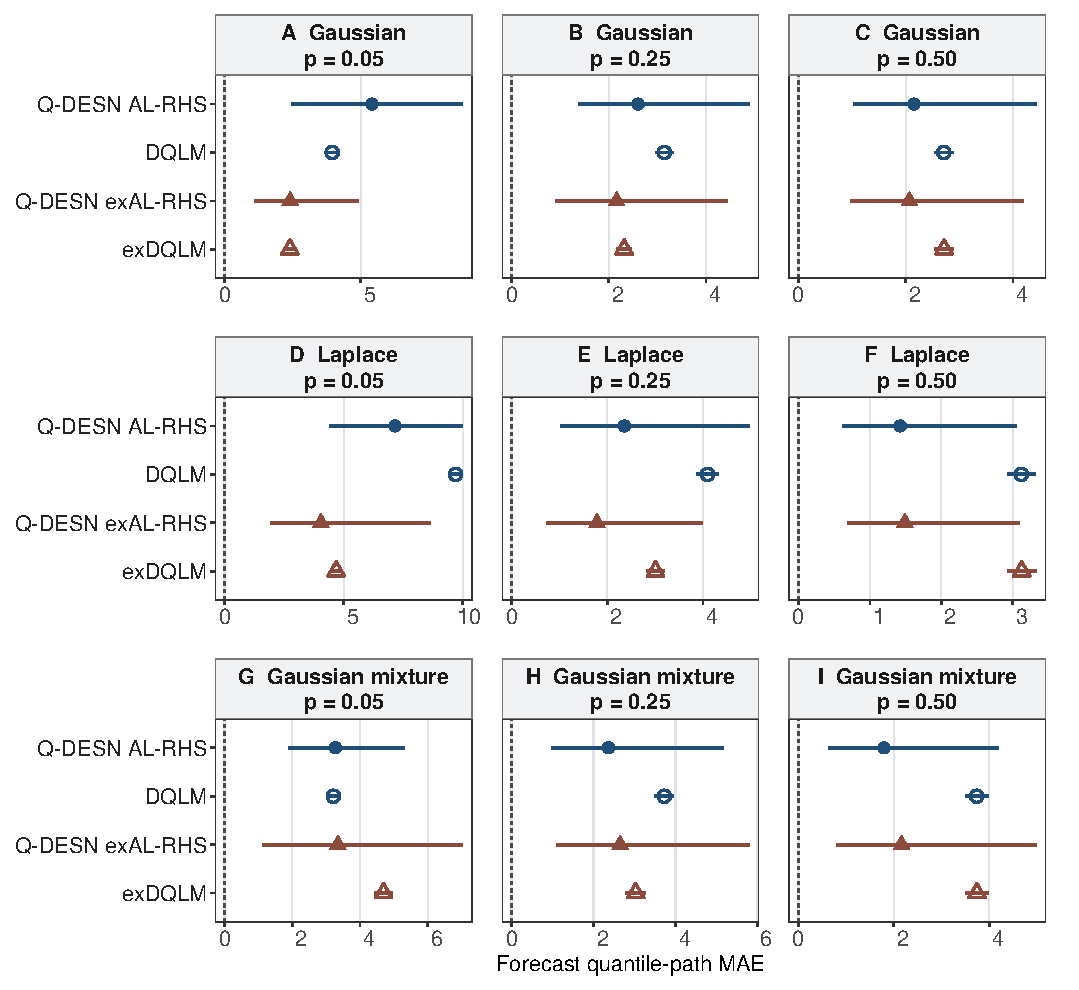
\includegraphics[width=0.98\textwidth]{figures/independent_simulation/independent_train500_eval500_mcmc_forecast_mae_v1.pdf}
\caption{MCMC forecast quantile-path MAE over 500 targets (17 origins): draw-wise means and equal-tailed 95\% intervals. The final origin contributes 20 leads, others 30. Colours and symbols follow Figure~\ref{fig:simulation-500obs-mcmc-forecast-mae-intervals}; the dashed line marks exact recovery.}
\figalt{Nine panels compare four models using mean forecast quantile-path MAE and 95 percent intervals over 500 scored targets.}
\label{fig:independent-eval500-forecast_mae}
\end{figure}

\begin{figure}[!htbp]
\centering
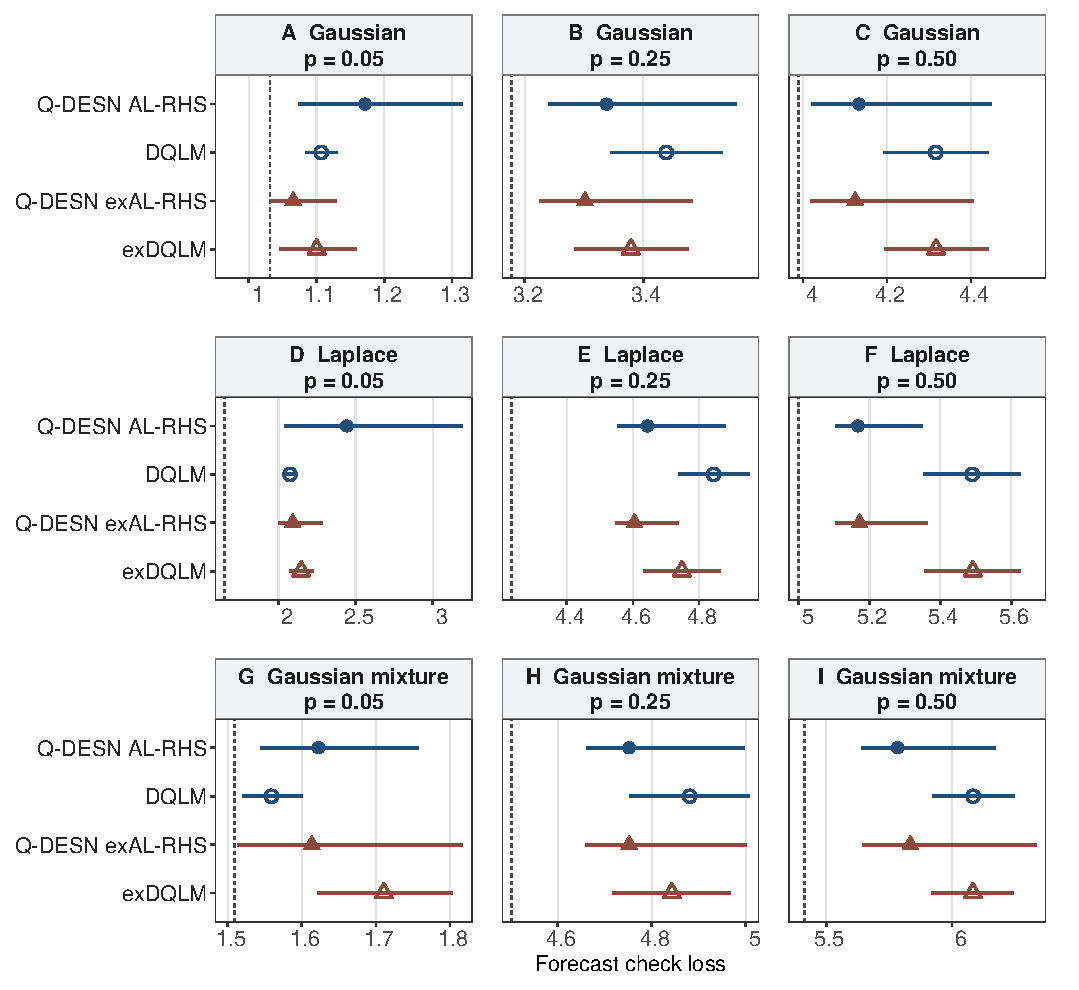
\includegraphics[width=0.98\textwidth]{figures/independent_simulation/independent_train500_eval500_mcmc_forecast_check_v1.pdf}
\caption{MCMC forecast check loss over the same 500 targets: draw-wise means and equal-tailed 95\% intervals. Colours and symbols follow Figure~\ref{fig:simulation-500obs-mcmc-forecast-mae-intervals}. The dashed line marks population expected check loss at the true conditional quantile, not a finite-sample lower bound.}
\figalt{Nine panels compare four models using mean forecast check loss and 95 percent intervals over 500 scored targets.}
\label{fig:independent-eval500-forecast_check}
\end{figure}
